\section{Analysis of the Problem}
\subsection{Clarification}
Based on the ten smart growth principles in `The Smart Growth Network'\cite{pdf:smart-growth}, a  smart growth metric is to be set up which can well measure how successfully a city develops.
With two mid-sized cities on two different continents selected, the problem including the following requirements can be solved:

\subsection{Requirement}
\begin{enumerate}
  \item Using the metric above, judge whether the current growth plan of each city obeys the `smart growth principles', and measure how successfully each city grows.
  \item Based on the geography, economic opportunities and prospective, work out a growth plan for each city under the smart metric, and sequence every factor in the order of potential.
  \item Revise the growth plan in \textbf{2}, given that the population changed by 50\% till 2050.
\end{enumerate}

%-------------------------------------%
%-------------------------------------%
%-------------------------------------%

\section{Introduction}
%由于不同城市的城市构成(包括道路网的建设、居民的生活工作习惯等)大相径庭,所以为了得到一个较为普适的城市发展评分标准,显然需要对城市进行一个适当的模型简化。在这里我们采用的是将城市划分为一个一个的square unit,同时对每个square unit定义其区域类别和发展程度。
%1933年的《雅典宪章》【加脚注或引用】提出城市应按居住、工作、游憩进行分区布置。在此基础上,我们将每个square unit的区域类别定义为如下五条之一:residential area、working area、recreation area、open space以及undeveloped。需要说明的是,working area主要包括了平时为居民提供生活服务的各类设施,如写字楼、加油站等;recreation则主要包括了可以为居民提供精神上的享受的设施,例如餐馆、图书馆、公园等;open space主要指的是开阔的自然景观(包括farmland),而undeveloped指的是可以在该区域进行开发改建。
Since different cities' compositions in detail (including transportation network, residents working habits) are quite different, in order to obtain a relatively universal metric standard for city development, we need to simplify actual cities into models properly.
In this paper, our method is to divide the city into multiple (2000 \~{} 3000) square units and define their types and development levels.
\\
In Athens Charter\footfullcite{conf:The-Athens-Charter}, it argues that city should be arranged according to its residencial, working and recreational function.
Based on that, we define each square unit's type as one of the followings:
\begin{itemize}
  \item residential area
  \item working area
  \item recreation area
  \item open space
  \item undeveloped area
\end{itemize}
Just to be clear, in our definition, working area contains all service facilities for residents' daily life, such as office buildings and gas stations.
Recreation area contains facilities that provide mentally enjoyment for residents, such as restrauts, libraries and parks.
Open space refers to open landscapes, including farmlands.
Undeveloped area refers to areas that can be developed in the future.
\\
%根据对smart growth principles的分条解读【脚注http://smartgrowth.org/smart-growth-principles/】,我们将十条principle合并为如下的四条准则:
According to our interpretation on the ten smart growth principles \cite{pdf:smart-growth}, we merge 10 principles into 4 judging standards.
\begin{enumerate}
  \item Mix Land Use
%这条准则包含了smart growth principles的第1,4,5条(我们用Pr.1, Pr.4, Pr.5表示第1,4,5条principle;后面将利用类似的记号)。主要原因是分区多样化方便了居民的出行,在土地混合多样使用的同时也能够提升社区本身的文化魅力。
  This standard contains the 1st, 4th and 5th smart growth principles (We denote them as Pr.1, Pr.2 and Pr.5, and we will use similar denotations in the following passage). The reason for using it is that `mix land use' facilitate residents' travelling and working, and improve communities' cultural attractions at the same time.
  \item Open Space and Landscape
%这条准则包含了Pr.2与Pr.6。根据smartgrowth.org上的解读,compact building design的重要目的之一是给居民提供宽阔的open space以提升舒适度,而第六条对于自然环境的保护事实上也与城市的自然景观密不可分。
  This standard contains Pr.2 and Pr.6. According to our interpretation, one of compact building design's most important goal is to provide residents with large open space to imporve their feeling of comfort. Natural protection in Pr.6 also has a tight connection with a city's open space and natural landscape.
  \item Housing Choice
%这条准则指的是Pr.3。我们需要为不同工资收入的人群提供与收入相符的住房选择的权利,这要求了working area附近有与之发展程度相近的residential area。
  This is standard refers to Pr.3. We need to provide different people with houses accordant with their income, which means there should be residential areas around each working area with a close development.
  \item Transportation Convenience
%这条准则指的是Pr.8。给市民多样的交通选择权利,这势必包含了公共交通的发达程度。出于量化考虑的角度,我们主要考虑公共交通的便利程度。
  This standard refers to Pr.8. To provide residents with more transportation choices, we must improve public transportation system. To measure transportation convenience, we mainly consider public transportation and its convenience.
\end{enumerate}
%对于Pr.7,Pr.9与Pr.10,由于它们的描述并不利于量化,我们将在之后制定growth plan中再对它们进行考虑,而不在metric的选择中对它们进行单独的考量。
As for Pr.7, Pr.9 and Pr.10. Since they are not easy to be quantified, we shall consider them when we make growth plans for cities, rather than set them as different metric.

%-------------------------------------%
%-------------------------------------%
%-------------------------------------%

\section{Assumptions}
\begin{itemize}
  \item \textbf{The side of each square unit measures 300 meters.}
  \item \textbf{Buildings in the same square unit has the same type and development.} Since the side length of a square unit is relatively short, the approximation is rational.
  \item \textbf{Except undeveloped areas, the development value in each square unit is a positive integer, generally no more than 3.}
  \item \textbf{Specifically, the development value in undeveloped area is zero.}
  \item \textbf{Averagely speaking, 10\% of all square units are open space.}
  \item \textbf{People in working areas and residential areas with the same development value are under the same financial condition.}
  \item \textbf{Each working area supports the same amout of people.}
  \item \textbf{Only undeveloped area and open space area with 1 development can be developed or redeveloped.}
\end{itemize}

%-------------------------------------%
%-------------------------------------%
%-------------------------------------%

\section{The two mid-sized cities}
\subsection{Gernal information}
We choose \textbf{Nottingham} in Great British and \textbf{Barrie} in Canada as our target cities.
To simplify the functional distribution, we divide the two cities into square units (300m $\times$ 300m).
With the help of Google map and OpenStreetMap, the following data is collected:
\begin{itemize}
  \item Functional type of the block
  \item Development level (between 1 and 3)
  \item Bus stop number (or other public transport station)
\end{itemize}
To put it simple, we have the following figure \ref{fig:two-cities} showing the distribution.
\begin{figure}[htbp]
  \label{fig:two-cities}
  \centering
  \subfigure[Barrie development]{
    \label{fig:subfigure:barrie-development}
    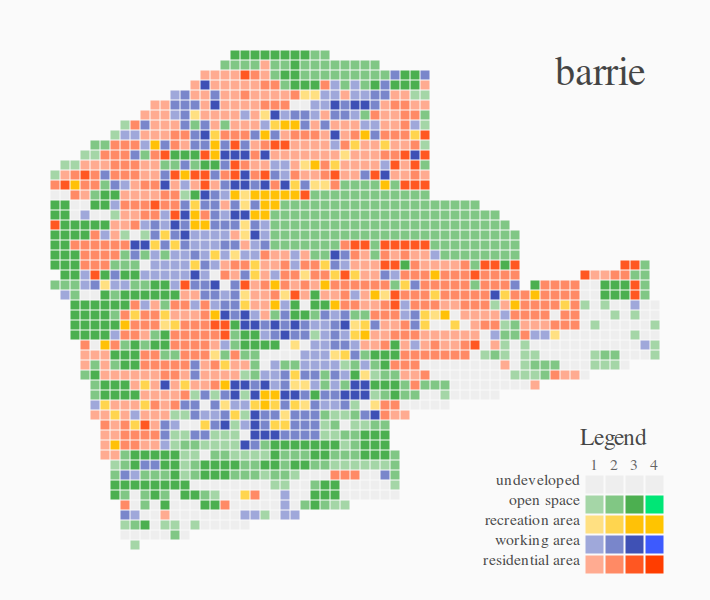
\includegraphics[width=6cm]{pic/barrie-development.png}
  }
  \subfigure[Barrie bus station]{
    \label{fig:subfigure:barrie-bus}
    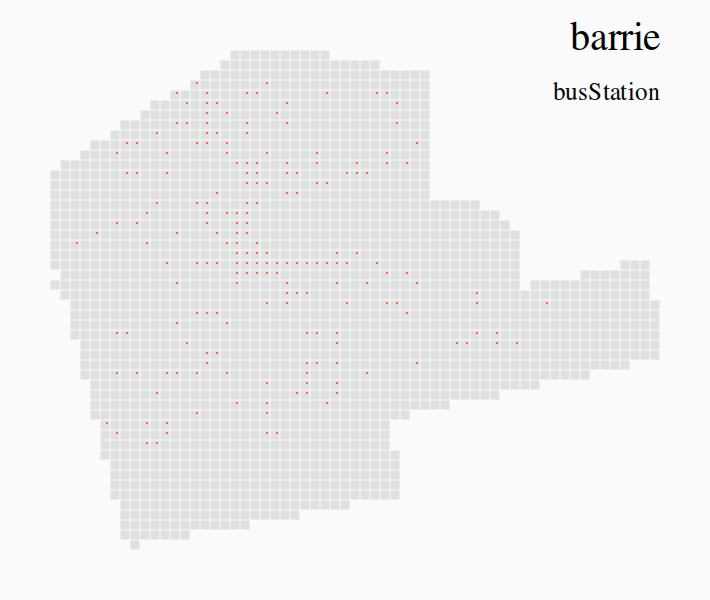
\includegraphics[width=6cm]{pic/barrie-busStation.png}
  }
  \subfigure[Nottingham development]{
    \label{fig:subfigure:nottingham-development}
    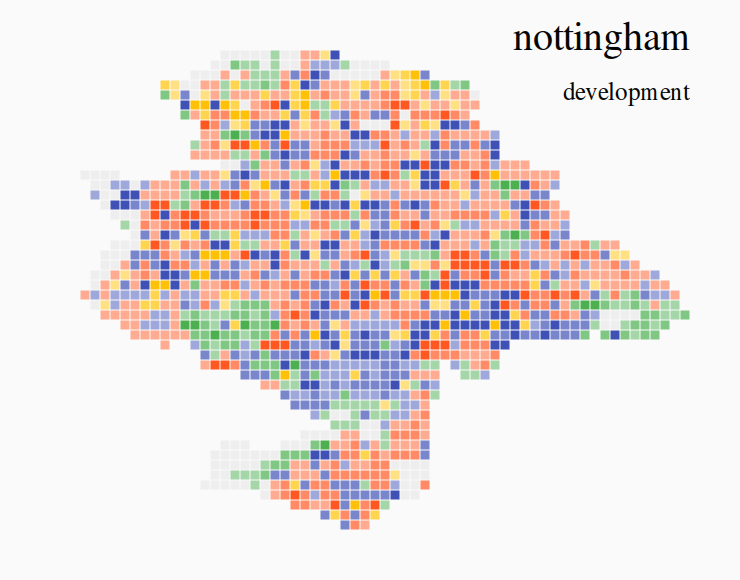
\includegraphics[width=6cm]{pic/nottingham-development.png}
  }
  \subfigure[Nottingham bus station]{
    \label{fig:subfigure:nottingham-bus}
    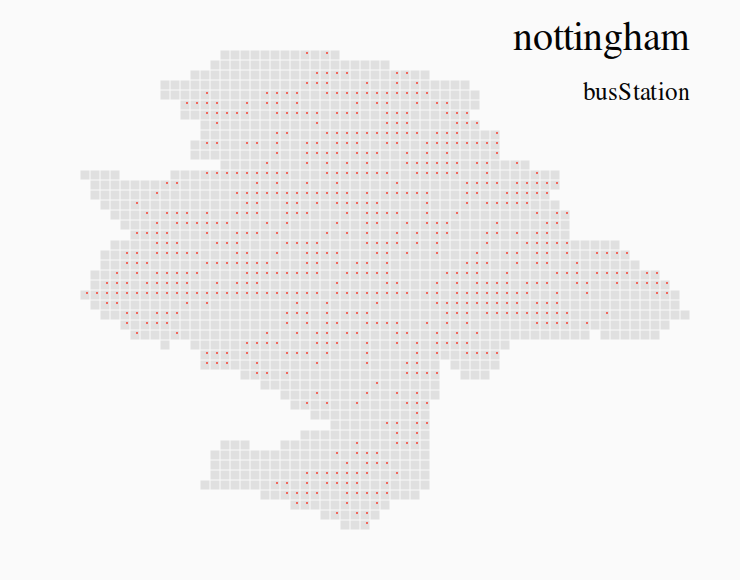
\includegraphics[width=6cm]{pic/nottingham-busStation.png}
  }
  \caption{}
\end{figure}

\subsection{Analysis of Nottingham}
\begin{table}
  \begin{tabular}{c|cccc}
    \hline
    Type & residential area & working area & recreation area & open space \\
    \hline
    Accounting for & 49.30\% & 32.07\% & 10.25\% & 13.96\% \\
    \hline
    Average level & 1.59 & 1.96 & 1.85 & 1.53 \\
    Average level*\footnote{(under government's plan)} & 1.66 & 2.28 & 2.05 & 1.53 \\
    \hline
  \end{tabular}
  \caption{Notthingham Distribution Data\footfullcite{pdf:the-nottingham-growth-plan}}
  \label{tab:nottingham-data}
\end{table}

As is shown in figure \ref{fig:subfigure:nottingham-development} \ref{fig:subfigure:nottingham-bus} and in table \ref{tab:nottingham-data}, the urban area of Nottingham city mainly consists of residential area, while open space accounts little.
It is worth noticing that working and recreational area has a relatively high development level, which is closely related to Nottingham's paying attention to technology, retail trade and advanced education.
However, it means that residential area has a lower development comparing to working area, indicating that the government's focus has long been on economic growth rather than people's happiness.
\\
\begin{table}
  \begin{tabular}{c|cccc|c}
    \hline
    Item & mix land use & beauty & residential choice & transport convenience & average \\
    \hline
    Score & 70.60 & 72.20 & 86.91 & 93.41 & 80.78 \\
    Score*\footnote{(under government's plan)} & 75.14 & 73.33 & 84.51 & 92.30 & 81.32 \\
    \hline
  \end{tabular}
  \caption{Notthingham Score under Smart Growth Metric}
  \label{tab:nottingham-score}
\end{table}
Combining data from table \ref{tab:nottingham-score} and distribution in figure \ref{fig:subfigure:nottingham-development} \ref{fig:subfigure:nottingham-bus}, we can find that working area contentrates in the middle part of the city's downtown, while residential and recreation area scatters around the downtown, which leads to a decrease in the score of mix land use.
As for the low performance in beauty, it seems contradictory to the temperate maritime climate, which is very suitable for plants to grow.
Nevertheless, if considering that Nottingham has a far more prosperous economy than the rest of Britain\footfullcite{wiki:nottingham-gdp}, it is not surprising that Notthingham, known as `a Technology City', inevitably sacrifices open space to give way to economic and technology development.
The low beauty score is against Principle 6, which emphasizes `critical environmental areas';
the convenient transport and diverse choices in residential area matches Principle 3 \& Principle 8.
\\
\begin{figure}[htb]
  \label{fig:nottingham-patch-diff}
  \centering
  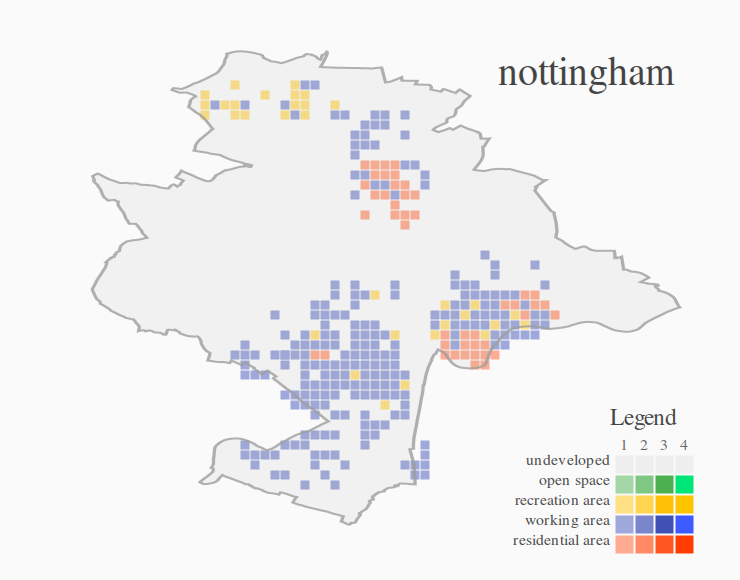
\includegraphics[width=6cm]{pic/nottingham-patch-diff-development.png}
  \caption{Nottingham development according to the government's plan}
\end{figure}
According to the government's growth plan and our smart growth metric, the city has some improvements, which is shown in figure \ref{fig:nottingham-patch-diff}.
It can be easily found that the following areas have a greater priority in the government's plan:
\begin{itemize}
  \item working area in downtown
  \item railway station neighbourhood
  \item northern residential and recreation area
\end{itemize}
To put it simple, the government still pays great attention to working area.
\\
As for the updated score under the government's plan in table \ref{tab:nottingham-data} and table \ref{tab:nottingham-score}, the residential choice score decreases due to the continuing ignorance of people's housing quality.
On the other hand, there is improvement in mix land use, for the sake of the development in the two area outside downtown.
\\
It is worth pointing out that, the growth plan we found doesn't refer to any development in open land; the file heavily depicts the techinal improvement for the city's landmarks - Boots and Biocity.
So it can be inferred that the government decides to further enhance the city's dominant industry.
The decision may meet its growth need to some extent, but it is still far from `Smart Growth Principle'.

\subsection{Analysis of Barrie}
\begin{table}
  \begin{tabular}{c|cccc}
    \hline
    Type & residential area & working area & recreation area & open space \\
    \hline
    Accounting for & 35.3\% & 20.97\% & 15.47\% & 36.30\% \\
    \hline
    Average level & 1.66 & 1.78 & 2.08 & 2.16 \\
    \hline
  \end{tabular}
  \caption{Barrie Distribution Data}
  \label{tab:barrie-data}
\end{table}

As is shown in figure \ref{fig:subfigure:barrie-development} \ref{fig:subfigure:barrie-bus} and in table \ref{tab:barrie-data}, working and recreation area has a rather small portion, while recreation area and open space develops much better than the rest.
The city of Barrie can be divided into three S-shape stripe zones: the left part is mostly residential, the middle part commercial, the right part mixing residents and recreation.
The high development of recreation area should owe to various winter-sport stadiums in the right zone, which is also a feature of city Barrie.
The heavy forest and large water area around the borderline of Barrie adds to the natural environment of the city's beauty; however, the heavy occupancy of land also forms an obstacle to the commercial development.
Comparing to Nottingham's terrian (see figure \ref{fig:subfigure:nottingham-development}), Barrie has a lower density of working area at the borderline, which may interfere with commercial communication.
\\
\begin{table}
  \begin{tabular}{c|cccc|c}
    \hline
    Item & mix land use & beauty & residential choice & transport convenience & average \\
    \hline
    Score & 54.24 & 92.11 & 64.06 & 50.67 & 65.27 \\
    Score*\footnote{(under government's plan)} & 57.93 & 92.50 & 62.73 & 57.70 & 67.72\\
    \hline
  \end{tabular}
  \caption{Barrie Score under Smart Growth Metric}
  \label{tab:barrie-score}
\end{table}
In table \ref{tab:barrie-score}, the first three scores reflects that the three `S-stipe zones' largely interrupts Barrie's adapting to `Principle 1'(mix land use) and housing choice in `Principle 3'.
It's worth mentioning that roads in Barrie are a lot wider (and the distribution is more discrete than in Nottingham), so people tenf to drive instead of taking a bus, which is contrary to diverse transport choices in `Principle 8'.
\\
We looked up for the plan of Barrie government \cite{pdf:barrie-downtown-plan} \cite{pdf:barrie-waterfront} \cite{pdf:barrie-official-plan} \cite{pdf:barrie-industrial-mapping} and arrange out the following improvements, shown in figure \ref{fig:barrie-patch-diff}.
\begin{figure}[htb]
  \label{fig:barrie-patch-diff}
  \centering
  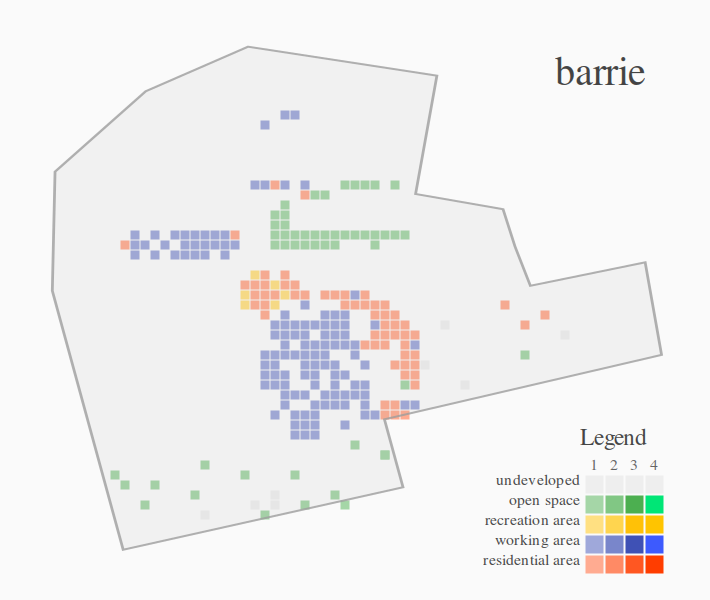
\includegraphics[width=6cm]{pic/barrie-patch-diff-development.png}
  \caption{Barrie development according to the government's plan}
\end{figure}
The government seems to have realized their ignorance in commercial, so the improvements concertrated in the mid S-stripe zone, the right stripe zone and at the same time improve the lake area.
It is obvious that the government still pays great attention to economic development, since 55.35\% efforts are made to working area.
The score under the government's plan is shown in table \ref{tab:barrie-score}.
\\
The government of Barrie seems to take a very different approach from that of Nottingham; it emphasizes its weak points rather than becoming a tourism city.
However, the S-shape stripe zones still largely interfere with the diverse development.
It is hard to make a big change in the city's functional distribution just in a short time of 10 years.

%-------------------------------------%
%-------------------------------------%
%-------------------------------------%

\section{Setting up the model}
%我们利用类似于坐标平面的方式来记录每个square unit,也就是每个square unit都可以被表示成【G3】的形式。后面的所有【G3】都是代表一个square unit。同时我们用【G6】表示【G3】的区域类别,【G8】表示【G3】的发展程度。
We record all square units in a plane coordinate system, which means every square unit can be represented as [G3].
Hereafter every [G3] represents a square unit.
Meanwhile, we use [G6] to represent [G3]'s area type and [G8] to represent [G3]'s development level.
\\
%需要指出的是,在下面的计算公式中都不考虑类别为unused area的square unit;unused area只是在之后的growth plan中有所涉及。
We point out that in the following formulas, unused areas are out of consideration. We will mention unused area in the growth plan part.
\\
%公式1
\subsection{Formula 1}
%首先我们对一个城市的分区多样化程度进行定量分析。由于Pr.4中鼓励create walkable neighborhoods,所以我们主要考量居民可以从residential area通过步行到达working area和recreation area。
%对于某一个square unit,我们考虑与之横纵坐标之差均不大于2的所有square unit;这样的话,居民只需要步行至多【G1】就可以到达自己所想要去的功能分区。所以对于,定义其mix-metric为【G2】,其中【G4】指的是【G5】相对于【G3】而言为分区多样化提供的贡献。
%容易看到,【G5】的发展程度越高,与【G3】的距离越近,多样化程度就越高。同时,两个区域类别对于分区多样化的贡献程度应该是不同的;这是因为对于一般的民众来说,working area靠近会更为重要一些。所以我们在metric中认为【G7】,这里【G9】表示不同的区域类别对于居民的重要程度。在我们的metric中,权值的取值可以见下表:
First of all, we consider how to measure the level of mix land use.
Since Pr.4 encourages to create walkable neighborhoods, we mainly consider working areas and recreation areas within a walkable distance from a residential area.
\\
As for a specific square unit, we consider other square units that satisfy [F].
In this case, residents only need to walk at most [G1] to reach their desired square unit.
So we define its mix-metric as [G2], where [G4] represents how much [G5] contributes to [G3]'s mix-land-use level.
\\
It's easy to note that the higher [G5]'s development level is and the closer [G5] is to [G3], the higher [G3]'s mix-metric scores.
However, the two different types of areas contribute differently to mix-land-use level.
To general residents, working areas are of more importance.
So in mix-metric, we suppose [G7], where [G9] represents the importance of different area types to residents. Details are in the following table.
\\
【G10】  residential area      working area      recreation area        open space
【G9】       0                     0.6                0.4                    0
\\
%最终城市的分区多样性指数便取决于所有residential area的mix-metric的加权平均值:【G11】。对每个residential area加权的原因是residential area的发展程度越高,分区多样性越显著,但不如working area那样明显。
%接下来我们需要将分区多样性指数换算成一个百分制的得分。
The city's mix-metric is decided by all residential areas' weighted average mix-metric [G11].
We use weighted means, because the higher residential area's development level is, the more mixed the city is, but not as prominent as working areas.
\\
Next we present a hundred-mark system to obtain a score.
\\
%我们引入一个调分函数【G12】:【G13】。【G12】满足当x趋向于正无穷时,函数的值趋向于100。
We define an adjust function [G12] : [G13]. [G12] satisfies that when x tends to infinity, its value tends to 100.
\\
%我们通过如下的准则来确认参数r,k的值:由于根据assumption,大多数建筑的发展程度都不超过3,所以我们认为当所有建筑的发展程度都是1时,分区多样性指数的期望值的得分为60分;而所有建筑的发展程度都是2时,分区多样性指数的期望值的得分为85分。
We now set the value of parameters r and k.
According to assumption, most areas' development level do not exceed 3, so we suppose when all areas' development level is 1, the city scores 60 and when all areas' development level is 2, the city scores 85.
\\
%当所有建筑的发展程度都是1时,分区多样性指数的期望值为【G14】;当所有建筑的发展程度都是1时,分区多样性指数的期望值为【G15】。
So, when all areas' development level equals to 1, the city's mix-land-use score is expected to be [G14].
When all areas' development level equals to 2, the expectation is [G15].
\\
%由此解得【G16】。
Thus we have [G16]
%于是城市的分布多样性得分为【G17】。
So the city's mix-land-use score is [G17].
\\

%公式2
\subsection{Formula 2}
%其次我们对一个城市的景观规划进行定量分析。注意到自然景观起到的主要作用事实上是改善了周边的城市分区的生活质量,所以对于每一个非open space的square unit【G3】,它所能受到自然景观的影响是【G18】(与之前确定【G7】时一样,自然景观的影响与自然景观的发展程度正相关,而与距离反相关)。
Secondly, we measure a city's sight and landscape.
Awaring that in city, natural landscape's main affect is to improve quality of life in the neighborhood areas, so as for any non-open-space square unit, the affect on it by landscape is [G18].
(As previously obtained [G7], the metric is positive correlated with the open space's development level, and negative corellated with the distance between them)
\\
%所以一个城市的自然景观指数也就是所有b(i,j)的平均值,即【G19】。
So the city's beauty-metric is the average of all square units, i.e. [G19]
\\
%同样引入调分函数【G12】。与公式1完全类似,我们定义当所有open space的发展程度都是1时,景观指数的期望值的得分为60分;而所有open space的发展程度都是2时,景观指数的期望值的得分为85分。
We define another adjust function [G12], as above.
Similarly, we define when all areas' development level is 1, the city's beauty is expected to be 60, and when all areas' development level reaches 2, the expectation is 85.
\\
%当所有open space的发展程度都是1时,景观指数的期望值为【G20】;所有open space的发展程度都是2时,景观指数的期望值为【G21】。
So, when all areas' development level equals to 1, the city's mix-land-use score is expected to be [G20].
When all areas' development level equals to 2, the expectation is [G21].
\\
%由此解得【G22】。
Thus we have [G22].
%于是城市的景观得分为【G23】。
So the city's beauty score is [G23].
\\
%公式3
\subsection{Formula 3}
%接下来我们对一个城市的住房选择自由进行定量分析。对于在某个working area工作的人,他需要在自己的工作地点附近(与上面的讨论类似,我们依然认为与之横纵坐标之差均不大于2的square unit算作其附近)寻找一个与收入水平相符合的居住地点,也就是发展程度尽量接近的residential area。那么对于某个working area【G3】,在此工作的人的住房选择符合指数【G24】。由于发展程度都是正整数,所以可能的住房选择符合指数基本是有限的;所以这里我们不再引入调分函数【G12】,而是直接给出城市的住房选择自由得分【G25】。
Now, we consider how to measure a city's housing choice.
Particularly, consider a person in a working area, he needs to choose a residencial area around it (As above, we consider the same range of 5*5 areas) with a similar cost level, i.e. a residencial area with a similar development level.
As for a specific working area [G3], the housing-metric for people working there is [G24].
Since development level is a positive integer no more than 4, so housing-metric's value is limited.
Thus we don't use adjust function [G12], but directly define the area's housing score [G25].
\\
%这里,住房选择自由得分并不是直接对于所有working area计算均分,而应该是对所有工作的人进行计算均分;只是根据我们的assumption,我们简化地认为所有人的工作地点平均分布在了working area中。
Note that we don't define the city's housing score as the average of all working areas' housing scores, but by all people working in the area(the higher the development is, the more people are working there).
According to our assumption, we simply suppose all people in a working area are well-distributed.
\\

%公式4
\subsection{Formula 4}
%一般来说,一个城市的公共交通线路的互相换行是较为容易的。所以,我们在考察交通便利程度的时候,仅考虑每个square unit附近是否有公交站点;所以如果一个square unit附近的square unit中有至少一个建有公交站点,那么称之为convenient。最终的交通便捷得分即等于convenient的square unit占square unit的总数的百分数。
Generally speaking, changing lines in a city's public transportation system is relatively easy.
So when we consider a city's transportation-metric, we only consider whether there exists a bus station in a square unit.
If in a square unit's neighborhood (in this case, 3*3 neighborhood) there exists a bus station, we say the square unit is convenien.
The transportation score is then defined as [F].
\\
%在后面的评定之中,我们会对城市计算如上的四个得分的平均分,作为该城市的综合得分。但是需要指出的是,这个综合得分只能粗略地代表这个城市是否遵循了所有的smart growth principle。由于四项得分折合成百分制的标准不尽统一,所以这个综合得分只是作为评判的一个参考,而四项分别的得分才是我们分析城市并判断其发展侧重点的重要指标。
In the following evaluation, we calculate the average score of the four scores above as the city's overall score.
But it is neccessary to mention that this overall score only roughly represents whether this city follows all smart growth principles.
Since the four scores are not concordant, we should take more notice of the four scores separately to evaluate a city's growth and its focus points.
\\

%-------------------------------------%
%-------------------------------------%
%-------------------------------------%


\printbibliography

%-------------------------------------%
%-------------------------------------%
%-------------------------------------%
